% -*- LaTeX -*-
% -*- coding: utf-8 -*-
%
% ~~~~~~~~~~~~~~~~~~~~~~~~~~~~~~~~~~~~~~~~~~~~~~~~~~~~~~~~~~~~~~~~~~~~~~~~~~~~~~
%
%                             michael a.g. aïvázis
%                      california institute of technology
%                      (c) 1998-2010  all rights reserved
%
% ~~~~~~~~~~~~~~~~~~~~~~~~~~~~~~~~~~~~~~~~~~~~~~~~~~~~~~~~~~~~~~~~~~~~~~~~~~~~~~
%

\lecture{Introduction to parallel programming models}{20100111}

% --------------------------------------
% generic parallel architecture
\begin{frame}[fragile]
%
  \frametitle{Impact of architecture on algorithm design}
%
  \begin{itemize}
%
    \item recall the five steps of parallel algorithm design
      \begin{itemize}
      \item identification of the parallelizable part, partitioning into fine grain tasks,
        examination of the task communication patterns, task coarsening, and mapping coarse
        tasks onto processors
      \end{itemize}
%
    \item and the layout of the generic parallel architecture:
%
  \begin{figure}
    \centering
    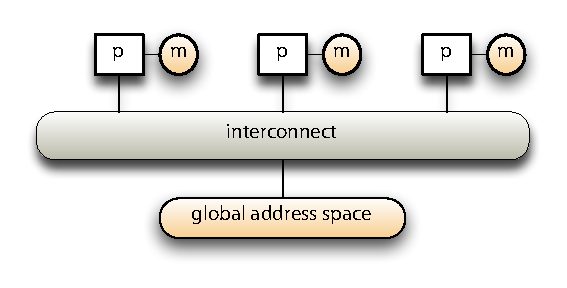
\includegraphics[width=.70\linewidth]{figures/generic-parallel-architecture.pdf}
    \label{fig:gpa-redux}
  \end{figure}
%
  \item let's move memory around and examine how this affects the programming model
  \item for a trivial but instructive problem
  \end{itemize}
%
\end{frame}

% --------------------------------------
% template
\begin{frame}[fragile]
%
  \frametitle{Parallel programming models}
%
  \begin{itemize}
%
  \item control
    \begin{itemize}
    \item how is parallelism {\em created}
    \item what is the {\em sequencing} of instruction streams in each task
    \item how do tasks {\em synchronize}
    \end{itemize}
%
    \item data address spaces
      \begin{itemize}
        \item what data is private to each task; what data must be shared
        \item how is logically shared data created, accessed or communicated, and synchronized
      \end{itemize}
%
    \item instruction sets
      \begin{itemize}
      \item what are the fundamental operations for process creation, communication,
        and synchronization
      \item which operations are {\em atomic}
      \end{itemize}
%
    \item cost
      \begin{itemize}
      \item how fast does it run
      \item are resources used efficiently
      \item how hard is it to code correctly
      \end{itemize}
%
  \end{itemize}
%
\end{frame}

% --------------------------------------
% problem setup
\begin{frame}[fragile]
%
  \frametitle{Embarrassingly parallel: $p$ processor reduction}
%
  \begin{itemize}
%
  \item given a function $f$ and a sequence of numbers $S$ of length $N$, evaluate the sum
    \[
    s = \sum_{i=0}^{N-1}f(S_{i})
    \]
%
  \item parallel tasks: the function evaluations, the computation of partial sums
%
  \item strategy: assign $n/p$ numbers to each processor
    \begin{itemize}
      \item each processor performs $n/p$ evaluations of $f$
      \item each processor computes its own partial sum
      \item one(?) of them collects the $p$ partial sums, and computes the global sum $s$
    \end{itemize}
%
  \item two classes of data
    \begin{itemize}
      \item logically shared:
        \begin{itemize}
        \item the global sum
        \item the input sequence $S$
        \end{itemize}
      \item logically private:
        \begin{itemize}
          \item the evaluations of $f$ on the local subsequence
          \item the local partial sums (?)
        \end{itemize}
    \end{itemize}
%
  \end{itemize}
%
\end{frame}

% --------------------------------------
% machine model 1: a shared memory machine
\begin{frame}[fragile]
%
  \frametitle{Shared memory machines}
%
  \begin{itemize}
%
  \item processors are all connected to a large pool of shared memory with a global address
    space
  \item typically, each processor has some local cache, but no private memory
  \item {\em cost}: accessing the cache is {\em much} faster than main memory
    \begin{itemize}
      \item tune: the memory footprint of $n/p$ numbers should match cache size
    \end{itemize}
%
  \begin{figure}
    \centering
    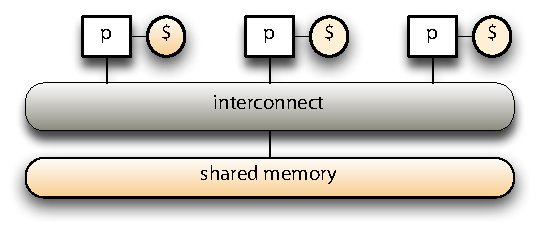
\includegraphics[width=.70\linewidth]{figures/shared-memory.pdf}
    \label{fig:shared-memory}
  \end{figure}
%
  \item for shared {\em address space} machine:
    \begin{itemize}
      \item replace caches with local/private memory
      \item cost: repeatedly accessed data should be copied to local storage
      \item not done much any more, but recently relevant thanks to hybrid CPU/GPGPU systems and
        the implementation details of nVidia chips
    \end{itemize}
%
  \end{itemize}
%
\end{frame}

% --------------------------------------
% programming a shared memory machine
\begin{frame}[fragile]
%
  \frametitle{Programming in a shared address space}
%
  \begin{itemize}
%
  \item the program creates and manages $p$ instruction streams (threads)
  \item each with a set of private variables
    \begin{itemize}
      \item registers, stack, cache
    \end{itemize}
%
  \item collectively with a set of shared variables
    \begin{itemize}
      \item statics, heap
    \end{itemize}
%
  \item communication is {\em implicit}: threads just access the shared memory locations
  \item synchronization is {\em explicit}: read/write flags, locks, semaphores
%
  \begin{figure}
    \centering
    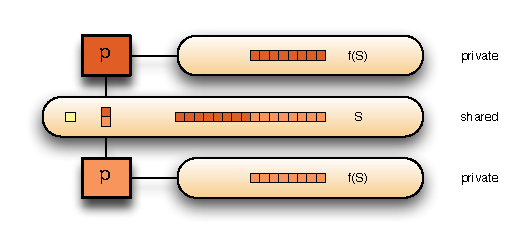
\includegraphics[width=\linewidth]{figures/reduction-shared.pdf}
    \label{fig:reduction-shared}
  \end{figure}
%
  \end{itemize}
%
\end{frame}

% --------------------------------------
% implementation of the reduction in a shared memory machine
\begin{frame}[fragile]
%
  \frametitle{Implementation in a shared address space}
%
  \begin{itemize}
%
  \item let's implement with two threads

    \vspace{.5em}
    \begin{minipage}{.40\linewidth}
      \begin{algorithm}[H]
%
        \footnotesize
        \DontPrintSemicolon
        \NoCaptionOfAlgo
        \SetAlCapHSkip{0ex}
%
        \caption{\hspace{1em}thread 1}
        \vspace{.5em}
%
        $s \leftarrow 0$ \;
        $s_{1} \leftarrow 0$ \;
        \For{$i \leftarrow 1$ \KwTo $n/2-1$}{
          $s_{1} \leftarrow s_{1} + f(S[i])$ \;
        }
        $s \leftarrow s+s_{1}$ \;
%
        \vspace{.5em}
%
      \end{algorithm}
    \end{minipage}
%
    \hspace{.1\linewidth}
%
    \begin{minipage}{.40\linewidth}
      \begin{algorithm}[H]
%
        \footnotesize
        \DontPrintSemicolon
        \NoCaptionOfAlgo
        \SetAlCapHSkip{0ex}
%
        \caption{\hspace{1em}thread 2}
        \vspace{.5em}
%
        $s \leftarrow 0$ \;
        $s_{2} \leftarrow 0$ \;
        \For{$i \leftarrow n/2$ \KwTo $n$}{
          $s_{2} \leftarrow s_{2} + f(S[i])$ \;
        }
        $s \leftarrow s+s_{2}$ \;
%
        \vspace{.5em}
      %
      \end{algorithm}
    \end{minipage}
    \vspace{.5em}
%
  \item what is wrong with this code? 
%
    \begin{itemize}
    \item {\em race condition}
    \item instructions from different threads can be executed in any order
    \item can you deduce all the possible values of $s$ after both threads finished executing?
    \item one possible solution is to place line 5 in a lock/load/modify/store/unlock block
    \end{itemize}
%
  \end{itemize}
%
\end{frame}

% --------------------------------------
% machine model 2: a distributed memory machine
\begin{frame}[fragile]
%
  \frametitle{Distributed memory machines}
%
  \begin{itemize}
%
  \item processors are all connected to their own private memory
  \item processors have no access to each other's memory, except through explicit exchanges
  \item each node is connected to a communication substrate: ethernet, myrinet, infiniband
%
  \begin{figure}
    \centering
    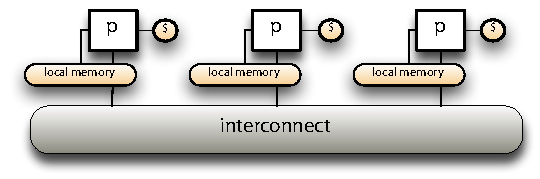
\includegraphics[width=.90\linewidth]{figures/distributed-memory.pdf}
    \label{fig:distributed-memory}
  \end{figure}
%
  \item all communication and synchronization is carried over the interconnect 
%
  \end{itemize}
%
\end{frame}

% --------------------------------------
% programming a distributed memory machine
\begin{frame}[fragile]
%
  \frametitle{Programming in a distributed address space}
%
  \begin{itemize}
%
  \item message passing
    \begin{itemize}
      \item programs consists of a collection of $n$ {\em named} processes
        \begin{itemize}
        \item typically numbered 0 through $n-1$
        \item thread of control, local address space
        \item local variables, statics, heap
        \end{itemize}
      \item processes communicate via {\em explicit} data exchanges
        \begin{itemize}
        \item matching pair of send/receive by source and destination processors respectively
        \item primitives for efficient implementation of many-to-many exchanges
        \end{itemize}
      \item co\"ordination is implicit in every communication
      \item logically shared data must be {\em partitioned} among the local processes
    \end{itemize}
%
  \item standard libraries: MPI, the survivor
%
  \begin{figure}
    \centering
    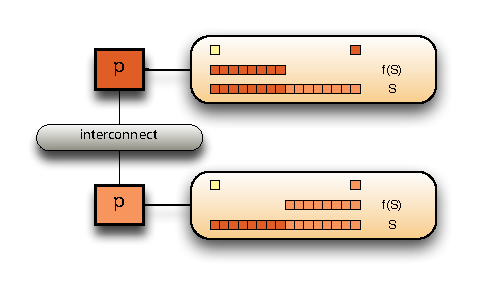
\includegraphics[width=.5\linewidth]{figures/reduction-distributed.pdf}
    \label{fig:reduction-distributed}
  \end{figure}
%
  \end{itemize}
%
\end{frame}

% --------------------------------------
% implementation of the reduction in a distributed memory machine
\begin{frame}[fragile]
%
  \frametitle{Implementation in a distributed address space}
%
  \begin{itemize}
%
  \item na\"ive implementation

    \vspace{.5em}
    \begin{minipage}{.40\linewidth}
      \begin{algorithm}[H]
%
        \footnotesize
        \DontPrintSemicolon
        \NoCaptionOfAlgo
        \SetAlCapHSkip{0ex}
%
        \caption{\hspace{1em}processor 1}
        \vspace{.5em}
%
        $s_{1} \leftarrow 0$ \;
        \For{$i \leftarrow 1$ \KwTo $n/2-1$}{
          $s_{1} \leftarrow s_{1} + f(S[i])$ \;
        }
        \KwSend $s_{1}$ \KwTo $p_{2}$ \;
        $s_{2} \leftarrow \KwRecv\ \KwFrom\ p_{2}$ \;
        $s \leftarrow s_{1}+s_{2}$ \;
%
        \vspace{.5em}
%
      \end{algorithm}
    \end{minipage}
%
    \hspace{.1\linewidth}
%
    \begin{minipage}{.40\linewidth}
      \begin{algorithm}[H]
%
        \footnotesize
        \DontPrintSemicolon
        \NoCaptionOfAlgo
        \SetAlCapHSkip{0ex}
%
        \caption{\hspace{1em}processor 2}
        \vspace{.5em}
%
        $s_{2} \leftarrow 0$ \;
        \For{$i \leftarrow n/2$ \KwTo $n$}{
          $s_{2} \leftarrow s_{2} + f(S[i])$ \;
        }
        \KwSend $s_{2}$ \KwTo $p_{1}$ \;
        $s_{1} \leftarrow \KwRecv\ \KwFrom\ p_{1}$ \;
        $s \leftarrow s_{2}+s_{1}$ \;
%
        \vspace{.5em}
      %
      \end{algorithm}
    \end{minipage}
    \vspace{.5em}
%
  \item what is wrong with this code? 
%
    \begin{itemize}
    \item {\em race condition}; more subtle than before
    \item send may block until a matching receive is executed  
    \end{itemize}
  \item options:
    \begin{itemize}
    \item pair up sends and receives to create logically atomic exchanges
    \item use non-blocking or asynchronous primitives
    \item use a many-to-many communication primitive, if available
    \end{itemize}
%
  \end{itemize}
%
\end{frame}

% --------------------------------------
% machine model 3: SIMD
\begin{frame}[fragile]
%
  \frametitle{SIMD machines}
%
  \begin{itemize}
%
  \item a large number of small, special purpose processors
%
  \item a single ``controller'' manages the instruction stream
    \begin{itemize}
      \item each processor executes the same instruction on its local data
      \item may be able  to specify which processors are active/idle
    \end{itemize}
%
  \begin{figure}
    \centering
    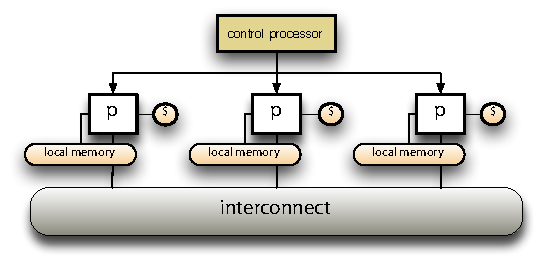
\includegraphics[width=.70\linewidth]{figures/simd.pdf}
    \label{fig:simd}
  \end{figure}
%
  \item hardware of this type fell out favor years ago
    \begin{itemize}
      \item but the associated programming model is still popular
      \item implemented by mapping $n$-fold parallelism to $p$ processors
      \item mostly done by compilers, e.g.~{\em High Performance FORTRAN} (HPF)
    \end{itemize}
%
  \item relevant again thanks to the CPU+GPGPU hybrids, which have similar layout
%
  \end{itemize}
%
\end{frame}

% --------------------------------------
% programming a SIMD machine
\begin{frame}[fragile]
%
  \frametitle{Data parallel programming model}
%
  \begin{itemize}
%
  \item single instruction stream of {\em parallel} operations
  \item parallel operation applied to entire data structure
    \begin{itemize}
      \item you may be able to restrict the {\em range} of operations to some defined subset of
        the data
    \end{itemize}
  \item communication and synchronization are implicit in the definition of the parallel
    operators
%
  \begin{figure}
    \centering
    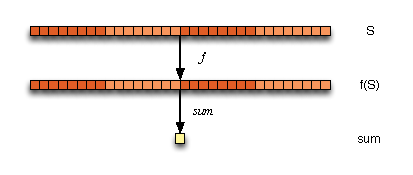
\includegraphics[scale=1.0]{figures/reduction-simd.pdf}
    \label{fig:reduction-simd}
  \end{figure}
%
  \item rather elegant, easy to understand, easy to reason about
  \item unfortunately, not all problems fit the paradigm nicely
  \item implemented by parallel functional languages, MATLAB
%
  \end{itemize}
%
\end{frame}

% --------------------------------------
% machine model 4: clusters
\begin{frame}[fragile]
%
  \frametitle{Clusters}
%
  \begin{itemize}
%
  \item commodity hardware configurations:
    \begin{itemize}
      \item CPUs with multiple cores: $2 \rightarrow 4 \rightarrow 6 \rightarrow 8 \rightarrow
        ?$
      \item motherboards with multiple CPUs
      \item sizeable memory on a single board
    \end{itemize}
%
  \item this hybrid is the current mainstream deployment: most of the Top500
%
  \item shared memory within a {\em blade}, message passing across blades
%
  \item there had to be an acronym: CLUMPs; fortunately no one uses it...
%
  \item programming models:
    \begin{itemize}
      \item treat machine as flat and always use message passing
        \begin{itemize}
        \item simple but ignores the performance characteristics of the memory hierarchy
        \item message passing library may be smart enough to switch between network and shared
          memory dynamically, e.g.~openMPI
        \end{itemize}
      \item expose both layers explicitly
        \begin{itemize}
          \item higher performance, but unpleasant to program
          \item hard to make portable
        \end{itemize}
    \end{itemize}
%
  \end{itemize}
%
\end{frame}

% --------------------------------------
% programming model 5: bulk synchronous
\begin{frame}[fragile]
%
  \frametitle{Bulk synchronous programming model}
%
  \begin{itemize}
%
  \item strategy that applies to both shared memory and message passing programming models
%
  \item program consists of interleaved {\em phases} synchronized by global barriers
    \begin{itemize}
      \item {\em compute} phases: all processors 
        \begin{itemize}
          \item operate on local data -- distributed memory
          \item operate with read access to global data -- shared memory
        \end{itemize}
      \item {\em communication} phases: all processors participate in data exchanges,
        rearrangements or reductions of global data
    \end{itemize}
%
    \item single program multiple data
      \begin{itemize}
        \item everybody is doing the same thing
        \item maps well to the structure of solutions of PDEs
          \begin{itemize}
            \item exchange data on processor partition boundaries 
            \item apply boundary conditions
            \item agree on a stable $\Delta t$ size (a global reduction)
            \item advance the solution by $\Delta t$
            \item repeat until you run out of time...
          \end{itemize}
      \end{itemize}
%
  \end{itemize}
%
\end{frame}

% --------------------------------------
% summary
\begin{frame}[fragile]
%
  \frametitle{Recap}
%
  \begin{itemize}
%
  \item in the early days, each machine was unique
    \begin{itemize}
      \item hardware, support for one programming model, perhaps a dedicated language with its
        compiler
%
      \item when a new machine came out you had to throw all your code away and start again
        \begin{itemize}
        \item ok for getting a thesis out, bad for building a career
        \end{itemize}
    \end{itemize}
%
  \item now we distinguish the programming model from the underlying hardware, so we can write
    portable, {\em correct} code that runs on large classes of machines
%
  \item unfortunately, writing {\em fast} code still requires tuning for some architectural
    details
    \begin{itemize}
      \item the design challenge is to simplify this process
      \item e.g., by exposing these details as user-configurable options that are determined at
        run-time
      \item best handled by {\em application frameworks}
    \end{itemize}
%
  \end{itemize}
%
\end{frame}

% --------------------------------------
% parallelization steps
\begin{frame}[fragile]
%
  \frametitle{Parallelization steps}
%
  \begin{figure}
    \centering
    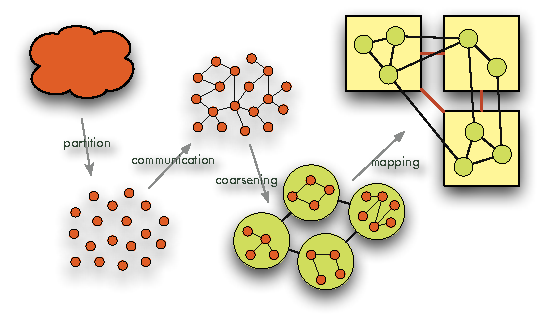
\includegraphics[scale=0.75]{figures/parallelization-steps.pdf}
    \label{fig:parallelization-steps}
  \end{figure}
  \vspace{-3.0em}
%
  \begin{itemize}
%
    \item steps in creating a parallel program
      \begin{itemize}
      \item identify the work that can be done in parallel
      \item partition it in terms of work units, the fine grain tasks
      \item analyze the communication patterns among work units
      \item coarsen into processes, the abstract entities that carry out tasks
      \item map to processors, the physical entities that execute the processes
      \end{itemize}
%
    \item goal: maximize the speedup due to parallelism
%
  \end{itemize}
%
\end{frame}

% --------------------------------------
% parallelizing reduction
\begin{frame}[fragile]
%
  \frametitle{Parallelizing our reduction example}
%
  \begin{itemize}
%
    \item for our example $s = \sum f(S)$
    \item partition into tasks
      \begin{itemize}
      \item computing each of the $F(S_{i})$
      \item $n$-fold parallelism, where ideally $n \gg p$ 
      \item computing the sum $s$
      \end{itemize}
%
    \item communication
      \begin{itemize}
        \item distribution of the initial input sequence $S$
        \item collection of the partial sums
      \end{itemize}
%
    \item coarsening: compute the partial sum of a cluster of evaluations
      \begin{itemize}
        \item thread $k$ sums up $s_{k} = \sum_{i = k n/p}^{(k+1)n/p 1} f(S_{i})$
        \item thread 1 sums up the partial results and communicates the result to the other
          threads
      \end{itemize}
%
    \item mapping: processor $i$ runs thread $i$
%
    \item at {\em runtime}
      \begin{itemize}
        \item start up the $p$ threads
        \item communicate/synchronize with thread 1
      \end{itemize}
%
  \end{itemize}
%
\end{frame}

% end of file 
